\documentclass{article}
\usepackage{graphicx} % Required for inserting images
\usepackage{fancyhdr} % Header
\usepackage{lastpage}
\usepackage[a4paper, total={6in, 8in}]{geometry}
\usepackage{float} % Floating position
\usepackage{hyperref} % Links
\usepackage{amsmath} % Math
\usepackage{amssymb} % Math
\usepackage{listings} % Import code in appendix
\usepackage{xcolor} % For coloring code
% Listing Configuration
\lstset{
    language=Python,
    basicstyle=\ttfamily\small,
    keywordstyle=\color{blue},
    stringstyle=\color{red},
    commentstyle=\color{green},
    showstringspaces=false,
    breaklines=true,
    frame=single
}
\usepackage{tikz} % Graph
\usetikzlibrary{bayesnet}
\usetikzlibrary{positioning}
\usetikzlibrary{decorations.markings}

\tikzset{
  red dot edge/.style={
    decoration={
      markings,
      mark=at position 0 with {\fill[red] circle (2pt);},
    },
    postaction={decorate},
  },
} % Red dot - place in [] just after \edge

\graphicspath{{images/}}

\newcommand{\authorFst}{Tristan Perrot}
\newcommand{\emailFst}{\href{mailto:tristanp@kth.se}{tristanp@kth.se}}
\newcommand{\authorSnd}{Étienne Riguet}
\newcommand{\emailSnd}{\href{mailto:riguet@kth.se}{riguet@kth.se}}

\pagestyle{fancy}
\fancyhf{} % clear all header and footer fields
\lhead{Assignment 1A \\ DD2434 - Machine Learning, Advanced Course}
\rhead{\authorFst \\ \authorSnd}
\cfoot{\thepage \  / \pageref{LastPage}}
\setlength{\headheight}{23pt}
\setlength{\footskip}{70pt}

\title{DD2434 - Machine Learning, Advanced Course \\ Assignment 1A}
\author{\authorFst \\ \emailFst \and \authorSnd \\ \emailSnd}
\date{November 2023}

\begin{document}

\maketitle

\begin{center}
    
\includegraphics[scale=0.5]{KTH_logo_RGB_bla.png}
\end{center}

\thispagestyle{empty}

\newpage
\tableofcontents
\newpage

\section{Exponential Family}

\subsection*{Question 1.1}

\begin{equation}
    \begin{split}
        p(x|\theta) & = h(x) \exp(\eta(\theta) \cdot T(x) - A(\eta))           \\
                    & = h(x) \exp(\eta(\lambda) \cdot T(x) - A(\eta(\lambda))) \\
                    & = h(x) \exp(\log \lambda \cdot x - A(\log \lambda))      \\
                    & = h(x) \exp(\log \lambda \cdot x - \lambda)              \\
                    & = h(x) \exp(\log \lambda \cdot x) \exp(-\lambda)         \\
                    & = e^{-\lambda} \frac{\lambda^x}{x!}
    \end{split}
\end{equation}

We can see that the distribution correspond to a \underline{Poisson distribution of parameter $\lambda$}.

\subsection*{Question 1.2}

\begin{equation}
    \begin{split}
        p(x|\theta) & = h(x) \exp(\eta(\theta) \cdot T(x) - A(\eta))                                            \\
                    & = \exp(\eta([\alpha, \beta]) \cdot [\log x, x] - A(\alpha - 1, -\beta))                   \\
                    & = \exp([\alpha - 1, -\beta] \cdot [\log x, x] - \log \Gamma(\alpha) + \alpha \log(\beta)) \\
                    & = \exp((\alpha - 1) \log x - \beta x - \log \Gamma(\alpha) + \alpha \log(\beta))          \\
                    & = \frac{\beta^\alpha}{\Gamma(\alpha)} x^{\alpha - 1} e^{-\beta x}
    \end{split}
\end{equation}

We can see that the distribution correspond to a \underline{Gamma distribution of parameters $\alpha$ and $\beta$}.

\subsection*{Question 1.3}

\begin{equation}
    \begin{split}
        p(x|\theta) & = h(x) \exp(\eta(\theta) \cdot T(x) - A(\eta))                                                                                                 \\
                    & = \frac{\exp(\eta([\mu, \sigma^2]) \cdot [x, x^2] - A(\eta([\mu, \sigma^2])))}{\sqrt{2 \pi}}                                                   \\
                    & = \frac{\exp([\frac{\mu}{\sigma^2}, - \frac{1}{2 \sigma^2}] \cdot [x, x^2] - A([\frac{\mu}{\sigma^2}, - \frac{1}{2 \sigma^2}]))}{\sqrt{2 \pi}} \\
                    & = \frac{\exp(\frac{\mu x}{\sigma^2} - \frac{x^2}{2 \sigma^2} - \frac{\mu^2}{2 \sigma^2} - \log \sigma)}{\sqrt{2 \pi}}                          \\
                    & = \frac{\exp(- \frac{(x - \mu)^2}{2 \sigma^2})}{\sigma \sqrt{2 \pi}}
    \end{split}
\end{equation}

We can see that the distribution correspond to a \underline{Normal distribution of parameters $\mu$ and $\sigma^2$}.

\subsection*{Question 1.4}

\begin{equation}
    \begin{split}
        p(x|\theta) & = h(x) \exp(\eta(\theta) \cdot T(x) - A(\eta))                        \\
                    & = 2 \exp(\eta(\lambda) \cdot x - A(\eta(\lambda)))                    \\
                    & = 2 \exp(- \lambda x - A(-\lambda))                                   \\
                    & = 2 \exp\left(- \lambda x + \log\left(\frac{\lambda}{2}\right)\right) \\
                    & = \lambda e^{- \lambda x}
    \end{split}
\end{equation}

We can see that the distribution correspond to a \underline{Exponential distribution of parameter $\lambda$}.

\subsection*{Question 1.5}

\begin{equation}
    \begin{split}
        p(x|\theta) & = h(x) \exp(\eta(\theta) \cdot T(x) - A(\eta))                                                                                     \\
                    & = \exp(\eta([\psi_1, \psi_2]) \cdot [\log x, \log (1 - x)] - A(\eta([\psi_1, \psi_2])))                                            \\
                    & = \exp([\psi_1 - 1, \psi_2 - 1] \cdot [\log x, \log (1 - x)] - A([\psi_1 - 1, \psi_2 - 1]))                                        \\
                    & = \exp((\psi_1 - 1) \log x + (\psi_2 - 1) \log (1 - x) - \log \Gamma(\psi_1) - \log \Gamma(\psi_2) + \log \Gamma(\psi_1 + \psi_2)) \\
                    & = \frac{\Gamma(\psi_1 + \psi_2)}{\Gamma(\psi_1) \Gamma(\psi_2)} x^{\psi_1 - 1} (1 - x)^{\psi_2 - 1}
    \end{split}
\end{equation}

We can see that the distribution correspond to a \underline{Beta distribution of parameters $\psi_1$ and $\psi_2$}.

\section{Dependencies in a Directed Graphical Model}

\subsection*{Question 2.6}

\begin{figure}[H]
    \centering
    \begin{tikzpicture}

  % Define nodes
  \node[latent] (theta) {$\theta_d$};
  \node[latent, left=of theta] (alpha) {$\alpha$};
  \node[latent, right=of theta] (z) {$Z_{d,n}$};
  \node[latent, right=of z] (w) {$W_{d,n}$};
  \node[latent, right=of w] (beta) {$\beta_k$};
  \node[latent, right=of beta] (eta) {$\eta$};

  % Connect nodes
  \edge {alpha} {theta}
  \edge {theta} {z}
  \edge {z} {w}
  \edge {beta} {w}
  \edge {eta} {beta}

  % Plates
  \plate [inner xsep=0.3cm] {plate1} {(z)(w)} {$N$}
  \plate [inner xsep=0.3cm] {plate2} {(theta)(z)(w)(plate1)} {$D$}
  \plate [inner xsep=0.2cm, xshift=0.1cm] {plate3} {(beta)} {$K$}

\end{tikzpicture}

    \caption{Graphical model of \href{https://www.jmlr.org/papers/volume3/blei03a/blei03a.pdf}{smooth LDA}.}
    \label{fig:fig1}
\end{figure}

The Bayes net take this form :

\begin{figure}[H]
    \centering
    \begin{tikzpicture}

  % Define nodes
  \node[latent] (theta_1) {$\theta_1$};
  \node[obs, below=of theta_1] (theta_d) {$\theta_d$};
  \node[latent, below=of theta_d] (theta_d+1) {$\theta_{d+1}$};
  \node[latent, below=of theta_d+1] (theta_D) {$\theta_D$};
  
  \node[latent, left=of theta_d] (alpha) {$\alpha$};
  
  \node[latent, right=of theta_1] (z_1n) {$Z_{1,n}$};
  \node[latent, right=of theta_d] (z_dn) {$Z_{d,n}$};
  \node[latent, right=of theta_d+1] (z_d+1n) {$Z_{d+1,n}$};
  \node[latent, right=of theta_D] (z_Dn) {$Z_{D,n}$};
  
  \node[latent, right=of z_1n] (w_1n) {$W_{1,n}$};
  \node[latent, right=of z_dn] (w_dn) {$W_{d,n}$};
  \node[latent, right=of z_d+1n] (w_d+1n) {$W_{d+1,n}$};
  \node[latent, right=of z_Dn] (w_Dn) {$W_{D,n}$};
  
  \node[obs, right=of w_d+1n] (beta) {$\beta_k$};

  \node[latent, right=of beta] (eta) {$\eta$};

  % Connect nodes
  \edge {alpha} {theta_1, theta_d, theta_d+1, theta_D}

  \edge {theta_1} {z_1n}
  \edge {theta_d} {z_dn}
  \edge {theta_d+1} {z_d+1n}
  \edge {theta_D} {z_Dn}

  \draw[dotted] (theta_1) -- (theta_d);
  \draw[dotted] (theta_d) -- (theta_d+1);
  \draw[dotted] (theta_d+1) -- (theta_D);

  \edge {z_1n} {w_1n}
  \edge {z_dn} {w_dn}
  \edge {z_d+1n} {w_d+1n}
  \edge {z_Dn} {w_Dn}

  \edge {beta} {w_1n, w_dn, w_d+1n, w_Dn}

  \edge {eta} {beta}

  % Plates
  \plate[inner xsep=0.2cm, xshift=0.1cm] {plate3} {(beta)} {$K$}
  \plate[inner xsep=0.3cm] {plate1} {(z_1n)(z_dn)(z_d+1n)(z_Dn)(w_1n)(w_dn)(w_d+1n)(w_Dn)} {$N$}

\end{tikzpicture}

    \label{fig:fig1.2.6.1}
\end{figure}

Then, if we use the method using the d-separation, we obtain this :

\begin{figure}[H]
    \centering
    \begin{tikzpicture}

  % Define nodes
  \node[latent] (theta_1) {$\theta_1$};
  \node[obs, below=of theta_1] (theta_d) {$\theta_d$};
  \node[latent, below=of theta_d] (theta_d+1) {$\theta_{d+1}$};
  \node[latent, below=of theta_d+1] (theta_D) {$\theta_D$};
  
  \node[latent, left=of theta_d] (alpha) {$\alpha$};
  
  \node[latent, right=of theta_1] (z_1n) {$Z_{1,n}$};
  \node[latent, right=of theta_d] (z_dn) {$Z_{d,n}$};
  \node[latent, right=of theta_d+1] (z_d+1n) {$Z_{d+1,n}$};
  \node[latent, right=of theta_D] (z_Dn) {$Z_{D,n}$};
  
  \node[latent, right=of z_1n] (w_1n) {$W_{1,n}$};
  \node[latent, right=of z_dn] (w_dn) {$W_{d,n}$};
  \node[latent, right=of z_d+1n] (w_d+1n) {$W_{d+1,n}$};
  \node[latent, right=of z_Dn] (w_Dn) {$W_{D,n}$};
  
  \node[obs, right=of w_d+1n] (beta) {$\beta_k$};

  \node[latent, right=of beta] (eta) {$\eta$};

  % Connect nodes
  \edge {alpha} {theta_1, theta_d, theta_d+1, theta_D}

  \edge {theta_1} {z_1n}
  \edge[red dot edge] {theta_d} {z_dn}
  \edge {theta_d+1} {z_d+1n}
  \edge {theta_D} {z_Dn}

  \draw[dotted] (theta_1) -- (theta_d);
  \draw[dotted] (theta_d) -- (theta_d+1);
  \draw[dotted] (theta_d+1) -- (theta_D);

  \edge {z_1n} {w_1n}
  \edge {z_dn} {w_dn}
  \edge {z_d+1n} {w_d+1n}
  \edge {z_Dn} {w_Dn}

  \edge[red dot edge] {beta} {w_1n, w_dn, w_d+1n, w_Dn}

  \edge {eta} {beta}

  % Plates
  \plate[inner xsep=0.2cm, xshift=0.1cm] {plate3} {(beta)} {$K$}
  \plate[inner xsep=0.3cm] {plate1} {(z_1n)(z_dn)(z_d+1n)(z_Dn)(w_1n)(w_dn)(w_d+1n)(w_Dn)} {$N$}

\end{tikzpicture}

    \label{fig:fig1.2.6.2}
\end{figure}

Therefore, we can see that $W_{d,n} \perp W_{d,n+1} | \theta_d, \beta_{1:K}$ is \underline{true}.

\subsection*{Question 2.7}

The Bayes net take this form (with d-separation marks) :
\begin{figure}[H]
    \centering
    \begin{tikzpicture}

  % Define nodes
  \node[latent] (theta_1) {$\theta_1$};
  \node[latent, below=of theta_1] (theta_d) {$\theta_d$};
  \node[latent, below=of theta_d] (theta_d+1) {$\theta_{d+1}$};
  \node[latent, below=of theta_d+1] (theta_D) {$\theta_D$};
  
  \node[latent, left=of theta_d] (alpha) {$\alpha$};
  
  \node[latent, right=of theta_1] (z_1n) {$Z_{1,n}$};
  \node[obs, right=of theta_d] (z_dn) {$Z_{d,n}$};
  \node[latent, right=of theta_d+1] (z_d+1n) {$Z_{d+1,n}$};
  \node[latent, right=of theta_D] (z_Dn) {$Z_{D,n}$};
  
  \node[latent, right=of z_1n] (w_1n) {$W_{1,n}$};
  \node[latent, right=of z_dn] (w_dn) {$W_{d,n}$};
  \node[latent, right=of z_d+1n] (w_d+1n) {$W_{d+1,n}$};
  \node[latent, right=of z_Dn] (w_Dn) {$W_{D,n}$};
  
  \node[latent, right=of w_d+1n] (beta) {$\beta_k$};

  \node[latent, right=of beta] (eta) {$\eta$};

  % Connect nodes
  \edge {alpha} {theta_1, theta_d, theta_d+1, theta_D}

  \edge {theta_1} {z_1n}
  \edge {theta_d} {z_dn}
  \edge {theta_d+1} {z_d+1n}
  \edge {theta_D} {z_Dn}

  \draw[dotted] (theta_1) -- (theta_d);
  \draw[dotted] (theta_d) -- (theta_d+1);
  \draw[dotted] (theta_d+1) -- (theta_D);

  \edge {z_1n} {w_1n}
  \edge [red dot edge] {z_dn} {w_dn}
  \edge {z_d+1n} {w_d+1n}
  \edge {z_Dn} {w_Dn}

  \edge {beta} {w_1n, w_dn, w_d+1n, w_Dn}

  \edge {eta} {beta}

  % Plates
  \plate[inner xsep=0.2cm, xshift=0.1cm] {plate3} {(beta)} {$K$}
  \plate[inner xsep=0.3cm] {plate1} {(z_1n)(z_dn)(z_d+1n)(z_Dn)(w_1n)(w_dn)(w_d+1n)(w_Dn)} {$N$}

\end{tikzpicture}

    \label{fig:fig1.2.7}
\end{figure}

Therefore, we can see that $\theta_{d} \perp \theta_{d+1} | Z_{d,1:N}$ is \underline{false}.

\subsection*{Question 2.8}

The Bayes net take this form (with d-separation marks) :
\begin{figure}[H]
    \centering
    \begin{tikzpicture}

  % Define nodes
  \node[latent] (theta_1) {$\theta_1$};
  \node[latent, below=of theta_1] (theta_d) {$\theta_d$};
  \node[latent, below=of theta_d] (theta_d+1) {$\theta_{d+1}$};
  \node[latent, below=of theta_d+1] (theta_D) {$\theta_D$};
  
  \node[obs, left=of theta_d] (alpha) {$\alpha$};
  
  \node[obs, right=of theta_1] (z_1n) {$Z_{1,n}$};
  \node[obs, right=of theta_d] (z_dn) {$Z_{d,n}$};
  \node[obs, right=of theta_d+1] (z_d+1n) {$Z_{d+1,n}$};
  \node[obs, right=of theta_D] (z_Dn) {$Z_{D,n}$};
  
  \node[latent, right=of z_1n] (w_1n) {$W_{1,n}$};
  \node[latent, right=of z_dn] (w_dn) {$W_{d,n}$};
  \node[latent, right=of z_d+1n] (w_d+1n) {$W_{d+1,n}$};
  \node[latent, right=of z_Dn] (w_Dn) {$W_{D,n}$};
  
  \node[latent, right=of w_d+1n] (beta) {$\beta_k$};

  \node[latent, right=of beta] (eta) {$\eta$};

  % Connect nodes
  \edge[red dot edge] {alpha} {theta_1, theta_d, theta_d+1, theta_D}

  \edge {theta_1} {z_1n}
  \edge {theta_d} {z_dn}
  \edge {theta_d+1} {z_d+1n}
  \edge {theta_D} {z_Dn}

  \draw[dotted] (theta_1) -- (theta_d);
  \draw[dotted] (theta_d) -- (theta_d+1);
  \draw[dotted] (theta_d+1) -- (theta_D);

  \edge[red dot edge] {z_1n} {w_1n}
  \edge[red dot edge] {z_dn} {w_dn}
  \edge[red dot edge] {z_d+1n} {w_d+1n}
  \edge[red dot edge] {z_Dn} {w_Dn}

  \edge {beta} {w_1n, w_dn, w_d+1n, w_Dn}

  \edge {eta} {beta}

  % Plates
  \plate[inner xsep=0.3cm] {plate1} {(z_1n)(z_dn)(z_d+1n)(z_Dn)(w_1n)(w_dn)(w_d+1n)(w_Dn)} {$N$}
  \plate[inner xsep=0.2cm, xshift=0.1cm] {plate3} {(beta)} {$K$}

\end{tikzpicture}

    \label{fig:fig1.2.8}
\end{figure}

Therefore, we can see that $\theta_{d} \perp \theta_{d+1} | \alpha, Z_{1:D,1:N}$ is \underline{true}.

\subsection*{Question 2.9}

\begin{figure}[H]
    \centering
    \begin{tikzpicture}

  % Define nodes
  \node[latent] (theta) {$\theta_d$};
  \node[latent, left=of theta] (alpha) {$\alpha$};
  \node[latent, below=of theta] (lambda) {$\Lambda_d$};
  \node[latent, left=of lambda] (phi) {$\Phi$};
  \node[latent, right=of theta] (z) {$Z_{d,n}$};
  \node[latent, right=of z] (w) {$W_{d,n}$};
  \node[latent, right=of w] (beta) {$\beta_k$};
  \node[latent, right=of beta] (eta) {$\eta$};

  % Connect nodes
  \edge {alpha} {theta}
  \edge {theta} {z}
  \edge {z} {w}
  \edge {beta} {w}
  \edge {eta} {beta}
  \edge {phi} {lambda}
  \edge {lambda} {theta}

  % Plates
  \plate [inner xsep=0.3cm] {plate1} {(z)(w)} {$N$}
  \plate [inner xsep=0.3cm] {plate2} {(theta)(lambda)(z)(w)(plate1)} {$D$}
  \plate [inner xsep=0.2cm, xshift=0.1cm] {plate3} {(beta)} {$K$}

\end{tikzpicture}

    \caption{Graphical model of \href{https://aclanthology.org/D09-1026.pdf}{Labeled LDA}.}
    \label{fig:fig2}
\end{figure}

The Bayes net take this form (with d-separation marks) :
\begin{figure}[H]
    \centering
    \begin{tikzpicture}

  % Define nodes
  \node[latent] (theta) {$\theta_d$};
  \node[latent, left=of theta] (alpha) {$\alpha$};
  \node[obs, below=of theta] (lambda) {$\Lambda_d$};
  \node[latent, left=of lambda] (phi) {$\Phi$};
  \node[latent, right=of theta] (z) {$Z_{d,n}$};
  \node[latent, right=of z] (w) {$W_{d,n}$};
  \node[obs, right=of w] (beta) {$\beta_k$};
  \node[latent, right=of beta] (eta) {$\eta$};

  % Connect nodes
  \edge {alpha} {theta}
  \edge {theta} {z}
  \edge {z} {w}
  \edge[red dot edge] {beta} {w}
  \edge {eta} {beta}
  \edge {phi} {lambda}
  \edge[red dot edge] {lambda} {theta}

  % Plates
  \plate[inner xsep=0.3cm] {plate1} {(z)(w)} {$N$}
  \plate[inner xsep=0.3cm] {plate2} {(theta)(lambda)(z)(w)(plate1)} {$D$}
  \plate[inner xsep=0.2cm, xshift=0.1cm] {plate3} {(beta)} {$K$}

\end{tikzpicture}

    \label{fig:fig1.2.9}
\end{figure}

Therefore, we can see that $W_{d,n} \perp W_{d,n+1} | \Lambda_d, \beta_{1:K}$ is \underline{false}.

\subsection*{Question 2.10}

The Bayes net take this form (with d-separation marks) :
\begin{figure}[H]
    \centering
    \begin{tikzpicture}

  % Define nodes
  \node[latent] (theta_1) {$\theta_1$};
  \node[latent, below=of theta_1] (theta_d) {$\theta_d$};
  \node[latent, below=of theta_d] (theta_d+1) {$\theta_{d+1}$};
  \node[latent, below=of theta_d+1] (theta_D) {$\theta_D$};
  
  \node[latent, left=of theta_d] (alpha) {$\alpha$};
  
  \node[latent, right=of theta_1] (z_1n) {$Z_{1,n}$};
  \node[obs, right=of theta_d] (z_dn) {$Z_{d,n}$};
  \node[obs, right=of theta_d+1] (z_d+1n) {$Z_{d+1,n}$};
  \node[latent, right=of theta_D] (z_Dn) {$Z_{D,n}$};
  
  \node[latent, right=of z_1n] (w_1n) {$W_{1,n}$};
  \node[latent, right=of z_dn] (w_dn) {$W_{d,n}$};
  \node[latent, right=of z_d+1n] (w_d+1n) {$W_{d+1,n}$};
  \node[latent, right=of z_Dn] (w_Dn) {$W_{D,n}$};
  
  \node[latent, right=of w_d+1n] (beta) {$\beta_k$};

  \node[latent, right=of beta] (eta) {$\eta$};

  \node[latent, below=of alpha] (lambda_1) {$\Lambda_1$};
  \node[latent, below=of lambda_1] (lambda_d) {$\Lambda_d$};
  \node[latent, below=of lambda_d] (lambda_d+1) {$\Lambda_{d+1}$};
  \node[latent, below=of lambda_d+1] (lambda_D) {$\Lambda_D$};
  \node[latent, left=of lambda_d] (phi) {$\Phi$};

  % Connect nodes
  \edge {alpha} {theta_1, theta_d, theta_d+1, theta_D}
  \edge {phi} {lambda_1, lambda_d, lambda_d+1, lambda_D}

  \edge {theta_1} {z_1n}
  \edge {theta_d} {z_dn}
  \edge {theta_d+1} {z_d+1n}
  \edge {theta_D} {z_Dn}

  \edge {lambda_1} {theta_1}
  \edge {lambda_d} {theta_d}
  \edge {lambda_d+1} {theta_d+1}
  \edge {lambda_D} {theta_D}

  \draw[dotted] (theta_1) -- (theta_d);
  \draw[dotted] (theta_d) -- (theta_d+1);
  \draw[dotted] (theta_d+1) -- (theta_D);

  \draw[dotted] (lambda_1) -- (lambda_d);
  \draw[dotted] (lambda_d) -- (lambda_d+1);
  \draw[dotted] (lambda_d+1) -- (lambda_D);

  \edge {z_1n} {w_1n}
  \edge[red dot edge] {z_dn} {w_dn}
  \edge[red dot edge] {z_d+1n} {w_d+1n}
  \edge {z_Dn} {w_Dn}

  \edge {beta} {w_1n, w_dn, w_d+1n, w_Dn}

  \edge {eta} {beta}

  % Plates
  \plate[inner xsep=0.3cm] {plate1} {(z_1n)(z_dn)(z_d+1n)(z_Dn)(w_1n)(w_dn)(w_d+1n)(w_Dn)} {$N$}
  \plate[inner xsep=0.2cm, xshift=0.1cm] {plate3} {(beta)} {$K$}

\end{tikzpicture}

    \label{fig:fig1.2.10}
\end{figure}

Therefore, we can see that $\theta_{d} \perp \theta_{d+1} | Z_{d,1:N}, Z_{d+1,1:N}$ is \underline{false}.

\subsection*{Question 2.11}

The Bayes net take this form (with d-separation marks) :
\begin{figure}[H]
    \centering
    \begin{tikzpicture}

  % Define nodes
  \node[latent] (theta_1) {$\theta_1$};
  \node[latent, below=of theta_1] (theta_d) {$\theta_d$};
  \node[latent, below=of theta_d] (theta_d+1) {$\theta_{d+1}$};
  \node[latent, below=of theta_d+1] (theta_D) {$\theta_D$};
  
  \node[latent, left=of theta_d] (alpha) {$\alpha$};
  
  \node[obs, right=of theta_1] (z_1n) {$Z_{1,n}$};
  \node[obs, right=of theta_d] (z_dn) {$Z_{d,n}$};
  \node[obs, right=of theta_d+1] (z_d+1n) {$Z_{d+1,n}$};
  \node[obs, right=of theta_D] (z_Dn) {$Z_{D,n}$};
  
  \node[latent, right=of z_1n] (w_1n) {$W_{1,n}$};
  \node[latent, right=of z_dn] (w_dn) {$W_{d,n}$};
  \node[latent, right=of z_d+1n] (w_d+1n) {$W_{d+1,n}$};
  \node[latent, right=of z_Dn] (w_Dn) {$W_{D,n}$};
  
  \node[latent, right=of w_d+1n] (beta) {$\beta_k$};

  \node[latent, right=of beta] (eta) {$\eta$};

  \node[latent, below=of alpha] (lambda_1) {$\Lambda_1$};
  \node[latent, below=of lambda_1] (lambda_d) {$\Lambda_d$};
  \node[latent, below=of lambda_d] (lambda_d+1) {$\Lambda_{d+1}$};
  \node[latent, below=of lambda_d+1] (lambda_D) {$\Lambda_D$};
  \node[obs, left=of lambda_d] (phi) {$\Phi$};

  % Connect nodes
  \edge {alpha} {theta_1, theta_d, theta_d+1, theta_D}
  \edge[red dot edge] {phi} {lambda_1, lambda_d, lambda_d+1, lambda_D}

  \edge {theta_1} {z_1n}
  \edge {theta_d} {z_dn}
  \edge {theta_d+1} {z_d+1n}
  \edge {theta_D} {z_Dn}

  \edge {lambda_1} {theta_1}
  \edge {lambda_d} {theta_d}
  \edge {lambda_d+1} {theta_d+1}
  \edge {lambda_D} {theta_D}

  \draw[dotted] (theta_1) -- (theta_d);
  \draw[dotted] (theta_d) -- (theta_d+1);
  \draw[dotted] (theta_d+1) -- (theta_D);

  \draw[dotted] (lambda_1) -- (lambda_d);
  \draw[dotted] (lambda_d) -- (lambda_d+1);
  \draw[dotted] (lambda_d+1) -- (lambda_D);

  \edge[red dot edge] {z_1n} {w_1n}
  \edge[red dot edge] {z_dn} {w_dn}
  \edge[red dot edge] {z_d+1n} {w_d+1n}
  \edge[red dot edge] {z_Dn} {w_Dn}

  \edge {beta} {w_1n, w_dn, w_d+1n, w_Dn}

  \edge {eta} {beta}

  % Plates
  \plate[inner xsep=0.3cm] {plate1} {(z_1n)(z_dn)(z_d+1n)(z_Dn)(w_1n)(w_dn)(w_d+1n)(w_Dn)} {$N$}
  \plate[inner xsep=0.2cm, xshift=0.1cm] {plate3} {(beta)} {$K$}

\end{tikzpicture}

    \label{fig:fig1.2.11}
\end{figure}

Therefore, we can see that $\Lambda_{d} \perp \Lambda_{d+1} | \Phi, Z_{1:D,1:N}$ is \underline{false}.

\section{CAVI}

\begin{figure}[H]
    \centering
    \begin{tikzpicture}

  % Define nodes
  \node[latent] (x) {$x$};
  \node[latent, above=of x] (mu) {$\mu$};
  \node[latent, right=of mu] (tau) {$\tau$};
  \node[above=of mu] (mu_0) {$\mu_0$};
  \node[left=of mu_0] (lambda_0) {$\lambda_0$};
  \node[above=of tau] (a_0) {$a_0$};
  \node[right=of a_0] (b_0) {$b_0$};

  % Connect nodes
  \edge {mu} {x}
  \edge {tau} {x}
  \edge {a_0} {tau}
  \edge {b_0} {tau}
  \edge {lambda_0} {mu}
  \edge {mu_0} {mu}

  % Plates
  \plate [inner xsep=0.3cm, inner ysep=0.3cm] {plate1} {(x)} {$N$}

\end{tikzpicture}

    \caption{DGM}
    \label{fig:fig3}
\end{figure}

\subsection*{Question 3.12}

In the bishop book, we can see that :

\begin{equation}
    p(X|\mu, \tau) = \left(\frac{\tau}{2\pi}\right)^{N/2} \exp\left\{-\frac{\tau}{2}\sum_{n=1}^{N}(x_n - \mu)^2\right\}
\end{equation}

\begin{equation}
    p(\mu|\tau) = \mathcal{N}(\mu|\mu_0, (\lambda_0 \tau)^{-1})
\end{equation}

\begin{equation}
    p(\tau) = \text{Gam}(\tau|a_0, b_0)
\end{equation}

Then, by using the code in appendix \ref{appendix:code.3.12}, we obtain :

\begin{figure}[H]
    \centering
    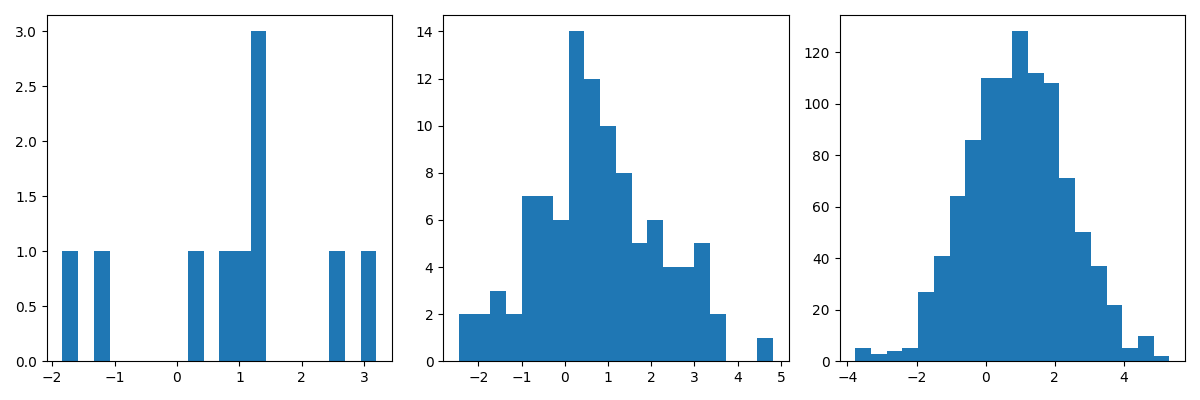
\includegraphics[scale=0.5]{images/12_data.png}
    \caption{Generated Data}
    \label{fig:3.12}
\end{figure}

\subsection*{Question 3.13}

Let's find the ML estimates of $\mu$ and $\tau$.
We know that $\log(q^*(\mu)) = \mathbb{E}_{-\mu}[\log p(X, \mu, \tau)]$.
Then, we can write :

\begin{equation}
    \begin{split}
        \log(q^*(\mu)) & = \mathbb{E}_{-\mu}[\log p(X, \mu, \tau)]                                                                                                                                                                                            \\
                       & \overset{+}{=} \mathbb{E}_\tau[\log p(X|\mu, \tau) + \log p(\mu|\tau)]                                                                                                                                                               \\
                       & = \mathbb{E}_\tau\left[\frac{N}{2}\log\left(\frac{\tau}{2\pi}\right) - \frac{\tau}{2}\sum_{n=1}^{N}(x_n - \mu)^2 + \frac{1}{2}\log\left(\frac{\lambda_0\tau}{2\pi}\right) - \frac{\lambda_0\tau}{2}\left(\mu - \mu_0\right)^2\right] \\
                       & \overset{+}{=} -\frac{\mathbb{E}_{\tau}[\tau]}{2}\left(\lambda_0 (\mu - \mu_0)^2 + \sum_{n=1}^{N}(x_n - \mu)^2\right)                                                                                                                \\
                       & = - \frac{\mathbb{E}_\tau[\tau]}{2}\left(\lambda_0\mu^2 - 2\lambda_0\mu\mu_0 + \lambda_0\mu_0^2 + \sum_{n=1}^{N}x_n^2 - 2\mu\sum_{n=1}^{N}x_n + N\mu^2\right)                                                                        \\
                       & = - \frac{\mathbb{E}_\tau[\tau]}{2}\left((\lambda_0 + N)\mu^2 - 2(\lambda_0\mu_0 + \sum_{n=1}^{N}x_n)\mu + \lambda_0\mu_0^2 + \sum_{n=1}^{N}x_n^2\right)                                                                             \\
                       & \overset{+}{=} - \frac{\mathbb{E}_\tau[\tau](\lambda_0 + N)}{2}\left(\mu^2 - 2\mu\frac{\lambda_0\mu_0 + \sum_{n=1}^{N}x_n}{\lambda_0 + N}\right)
    \end{split}
\end{equation}

Therefore we can conclude that $q^*(\mu) = \mathcal{N}(\mu|\mu_N, \lambda_N^{-1})$ with :
\begin{equation}
    \mu_N     = \frac{\lambda_0\mu_0 + \sum_{n=1}^{N}x_n}{\lambda_0 + N}
\end{equation}
\begin{equation}
    \lambda_N = (\lambda_0 + N)\mathbb{E}[\tau]
\end{equation}

And for $\tau$ we have :
\begin{equation}
    \begin{split}
        \log(q^*(\tau)) & = \mathbb{E}_{-\tau}[\log p(X, \mu, \tau)]                                                                                                                             \\
                        & \overset{+}{=} \mathbb{E}_\mu[\log p(X|\mu, \tau) + \log p(\mu|\tau)] + \log p(\tau)                                                                                   \\
                        & \overset{+}{=} (a_0 - 1)\log \tau - b_0\tau + \frac{N+1}{2}\log \tau - \frac{\tau}{2}\mathbb{E}_\mu\left[\sum_{n=1}^{N}(x_n - \mu)^2 + \lambda_0(\mu - \mu_0)^2\right] \\
                        & = (a_0 + \frac{N+1}{2} - 1)\log \tau - \left(b_0 + \frac{1}{2}\mathbb{E}_\mu\left[\sum_{n=1}^{N}(x_n - \mu)^2 + \lambda_0(\mu - \mu_0)^2\right]\right)\tau
    \end{split}
\end{equation}

Therefore we can conclude that $q^*(\tau) = \text{Gam}(\tau|a_N, b_N)$ with :
\begin{equation}
    a_N = a_0 + \frac{N+1}{2}
\end{equation}
\begin{equation}
    \begin{split}
        b_N & = b_0 + \frac{1}{2}\mathbb{E}_\mu\left[\sum_{n=1}^{N}(x_n - \mu)^2 + \lambda_0(\mu - \mu_0)^2\right]                                                                                                     \\
        b_N & = b_0 + \frac{1}{2}\left(\sum_{n=1}^{N}x_n^2 + N\mathbb{E}_\mu[\mu^2] - 2\mathbb{E}_\mu[\mu]\sum_{n=1}^{N}x_n + \lambda_0\left(\mathbb{E}_\mu[\mu^2] + \mu_0^2 - 2\mu_0\mathbb{E}_\mu[\mu]\right)\right) \\
    \end{split}
\end{equation}

With :
\begin{equation}
    \begin{split}
        \mathbb{E}_{q(\mu)}[\mu]   & = \mu_N                         \\
        \mathbb{E}_{q(\mu)}[\mu^2] & = \frac{1}{\lambda_N} + \mu_N^2 \\
        \mathbb{E}_{q(\tau)}[\tau] & = \frac{a_N}{b_N}
    \end{split}
\end{equation}

If we take non-informative priors then $a_0 = b_0 = \mu_0 = \lambda_0 = 0$, then we have :
\begin{equation}
    \begin{split}
        \mu_N     & = \overline{x}                                                      \\
        \lambda_N & = N\mathbb{E}[\tau]                                                 \\
        a_N       & = \frac{N+1}{2}                                                     \\
        b_N       & = \frac{1}{2}\mathbb{E}_\mu\left[\sum_{n=1}^{N}(x_n - \mu)^2\right]
    \end{split}
\end{equation}

And by using $\mathbb{E}[\tau] = \frac{a_N}{b_N}$ we obtain :
\begin{equation}
    \begin{split}
        \frac{1}{\mathbb{E}[\tau]} & = \frac{b_N}{a_N}                                                                             \\
        \frac{1}{\mathbb{E}[\tau]} & = \frac{2}{2(N+1)}\mathbb{E}_\mu\left[\sum_{n=1}^{N}(x_n - \mu)^2\right]                      \\
        \frac{1}{\mathbb{E}[\tau]} & = \frac{N}{N+1}\left(\overline{x^2} - 2\overline{x}\mathbb{E}[\mu] + \mathbb{E}[\mu^2]\right) \\
    \end{split}
\end{equation}

And, with the fact that $\mathbb{E}[\mu] = \mu_N$ and $\mathbb{E}[\mu^2] = \frac{1}{\lambda_N} + \mu_N^2$, we obtain :
\begin{equation}
    \begin{split}
        \mathbb{E}[\mu]   & = \overline{x}                                 \\
        \mathbb{E}[\mu^2] & = \frac{1}{N\mathbb{E}[\tau]} + \overline{x}^2
    \end{split}
\end{equation}

And therefore:
\begin{equation}
    \begin{split}
        \frac{1}{\mathbb{E}[\tau]} = \frac{N}{N+1}\left(\overline{x^2} - 2\overline{x}^2 + \frac{1}{N\mathbb{E}[\tau]} + \overline{x}^2\right) & \Leftrightarrow \frac{1}{\mathbb{E}[\tau]} - \frac{1}{(N+1)\mathbb{E}[\tau]} = \frac{N}{N+1}\left(\overline{x^2} - \overline{x}^2\right) \\
                                                                                                                                               & \Leftrightarrow \frac{N+1-1}{(N+1)\mathbb{E}[\tau]} = \frac{N}{N+1}\left(\overline{x^2} - \overline{x}^2\right)                          \\
                                                                                                                                               & \Leftrightarrow \frac{1}{\mathbb{E}[\tau]} = \left(\overline{x^2} - \overline{x}^2\right)                                                \\
                                                                                                                                               & \Leftrightarrow \frac{1}{\mathbb{E}[\tau]} = \frac{1}{N}\sum_{n=1}^{N}(x_n - \overline{x})^2                                             \\
    \end{split}
\end{equation}

Which define the ML estimates. The implementation is in the code in appendix \ref{appendix:code.3.13}.

\subsection*{Question 3.14}

The posterior is defined as $p(\mu, \tau|x)$. Then, we can write :
\begin{equation}
    \begin{split}
        p(\mu, \tau|x) & = \frac{p(x|\mu, \tau)p(\mu, \tau)}{p(x)} \\
                       & \propto p(x|\mu, \tau)p(\mu, \tau)
    \end{split}
\end{equation}

Where $x|\mu, \tau \thicksim \mathcal{N}(\mu|\mu, \tau^{-1})$ and $\mu, \tau \thicksim NormalGamma(\mu_0, \lambda_0, a_0, b_0)$.
Therefore, as we saw in the question 1.3 in the Module 1 exercise, we have $\mu, \tau|x \thicksim NormalGamma(\mu', \lambda', a', b')$, where :
\begin{equation}
    \begin{split}
        \mu'     & = \frac{N\overline{x} + \mu_0\lambda_0}{N + \lambda_0}                                                                                       \\
        \lambda' & = N + \lambda_0                                                                                                                              \\
        a'       & = a_0 + \frac{N-1}{2}                                                                                                                        \\
        b'       & = b_0 + \frac{1}{2}\left(\sum_{n=1}^{N}x_n^2 + \lambda_0\mu_0^2 - \frac{\left(N\overline{x} + \mu_0\lambda_0\right)^2}{N + \lambda_0}\right)
    \end{split}
\end{equation}

Therefore, if we plot the contour for each datasets we obtain :
\begin{figure}[H]
    \centering
    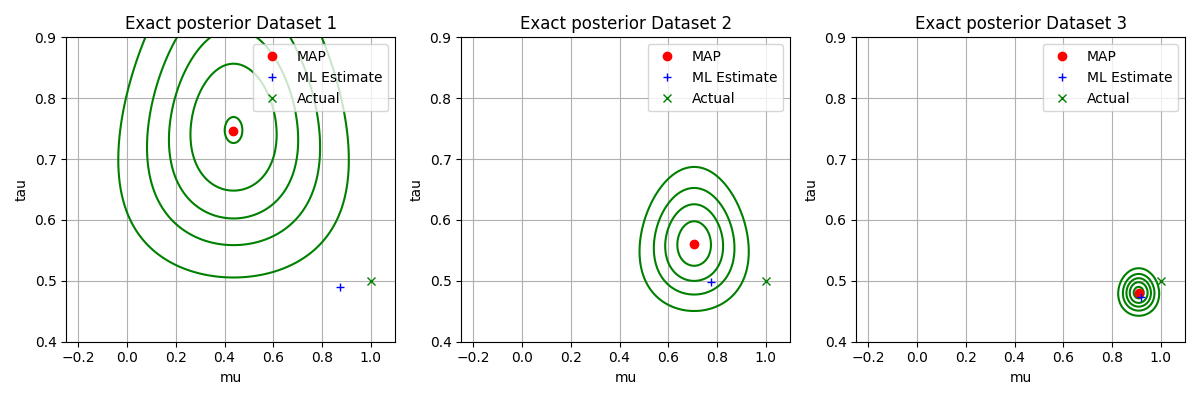
\includegraphics[scale=0.5]{images/14_contours.png}
    \caption{Contours of exact posteriors by datasets}
    \label{fig:3.14}
\end{figure}

The rest of the answer is in the code in appendix \ref{appendix:code.3.14}.

\subsection*{Question 3.15}

The equation (10.24) in the Bishop is the mean-field approximation which is :
\begin{equation}
    q(\mu, \tau) = q(\mu)q(\tau)
\end{equation}

This time, we take the result of the question 3.13 without setting the priors to 0.
Then, we have :
\begin{equation}
    \begin{split}
        q(\mu)  & = \mathcal{N}(\mu|\mu_N, \lambda_N^{-1}) \\
        q(\tau) & = \text{Gam}(\tau|a_N, b_N)
    \end{split}
\end{equation}

with updates equations in the cavi algorithm described by :
\begin{equation}
    \begin{split}
        \mu_N     & = \frac{\lambda_0\mu_0 + N\overline{x}}{\lambda_0 + N}                                                                                                                                                   \\
        \lambda_N & = (\lambda_0 + N)\mathbb{E}[\tau]                                                                                                                                                                        \\
        a_N       & = a_0 + \frac{N+1}{2}                                                                                                                                                                                    \\
        b_N       & = b_0 + \frac{1}{2}\left(\sum_{n=1}^{N}x_n^2 + N\mathbb{E}_\mu[\mu^2] - 2\mathbb{E}_\mu[\mu]\sum_{n=1}^{N}x_n + \lambda_0\left(\mathbb{E}_\mu[\mu^2] + \mu_0^2 - 2\mu_0\mathbb{E}_\mu[\mu]\right)\right)
    \end{split}
\end{equation}

and the expectations are the ones described in the equation (15).

Now, we need to find the ELBO formula :
\begin{equation}
    \begin{split}
        \mathcal{L}(q) & = \mathbb{E}_{q(\mu),q(\tau)}[\log p(X, \mu, \tau)] - \mathbb{E}_{q(\mu),q(\tau)}[\log q(\mu, \tau)]                                                                        \\
                       & = \mathbb{E}_{q(\mu),q(\tau)}[\log p(X|\mu, \tau) + \log p(\mu, \tau)] - \mathbb{E}_{q(\mu),q(\tau)}[\log q(\mu) + \log q(\tau)]                                            \\
                       & = \mathbb{E}_{q(\mu),q(\tau)}[\log p(X|\mu, \tau)] + \mathbb{E}_{q(\mu),q(\tau)}[\log p(\mu, \tau)] - \mathbb{E}_{q(\mu)}[\log q(\mu)] - \mathbb{E}_{q(\tau)}[\log q(\tau)] \\
                       & = \mathbb{E}_{q(\mu),q(\tau)}[\log p(X|\mu, \tau)] + \mathbb{E}_{q(\mu),q(\tau)}[\log p(\mu, \tau)] + \mathbb{H}_q[\mu] + \mathbb{H}_q[\tau]
    \end{split}
\end{equation}

If we compute the first term we have:
\begin{equation}
    \begin{split}
        \mathbb{E}_{q(\mu),q(\tau)}[\log p(X|\mu, \tau)] & = \mathbb{E}_{q(\mu),q(\tau)}\left[\frac{N}{2}\log\left(\frac{\tau}{2\pi}\right) - \frac{\tau}{2}\sum_{n=1}^{N}(x_n - \mu)^2\right]                                                                       \\
                                                         & = \frac{N}{2}\left(\mathbb{E}_{q(\tau)}[\log \tau] - \log(2\pi)\right)                                                                                                                                    \\
                                                         & \qquad\qquad - \frac{\mathbb{E}_{q(\tau)}[\tau]}{2}\left(\sum_{n=1}^{N}x_n^2 - 2\mathbb{E}_{q(\mu)}[\mu]N\overline{x_n} + N\mathbb{E}_{q(\mu)}[\mu^2]\right)                                              \\
                                                         & \overset{+}{=} \frac{N}{2}\mathbb{E}_{q(\tau)}[\log \tau] - \frac{\mathbb{E}_{q(\tau)}[\tau]}{2}\left(\sum_{n=1}^{N}x_n^2 - 2\mathbb{E}_{q(\mu)}[\mu]N\overline{x_n} + N\mathbb{E}_{q(\mu)}[\mu^2]\right) \\
    \end{split}
\end{equation}

And the second one is:
\begin{equation}
    \begin{split}
        \mathbb{E}_{q(\mu),q(\tau)}[\log p(\mu, \tau)] & = \mathbb{E}_{q(\mu),q(\tau)}\left[\log\left(\frac{b_0^{a_0} \sqrt{\lambda_0}}{\Gamma(a_0)\sqrt{2\pi}}\right) + (a_0 - \frac{1}{2})\log \tau - b_0\tau - \frac{\lambda_0\tau(\mu - \mu_0)^2}{2}\right]                              \\
                                                       & = \log\left(\frac{b_0^{a_0} \sqrt{\lambda_0}}{\Gamma(a_0)\sqrt{2\pi}}\right) + (a_0 - \frac{1}{2})\mathbb{E}_{q(\tau)}[\log \tau] - b_0\mathbb{E}_{q(\tau)}[\tau]                                                                   \\
                                                       & \qquad\qquad - \frac{\lambda_0\mathbb{E}_{q(\tau)}[\tau]}{2}\left(\mathbb{E}_{q(\mu)}[\mu^2] - 2\mu_0\mathbb{E}_{q(\mu)}[\mu] + \mu_0^2\right)                                                                                      \\
                                                       & \overset{+}{=} (a_0 - \frac{1}{2})\mathbb{E}_{q(\tau)}[\log \tau] - b_0\mathbb{E}_{q(\tau)}[\tau] - \frac{\lambda_0\mathbb{E}_{q(\tau)}[\tau]}{2}\left(\mathbb{E}_{q(\mu)}[\mu^2] - 2\mu_0\mathbb{E}_{q(\mu)}[\mu] + \mu_0^2\right) \\
    \end{split}
\end{equation}

And we can compute all of that because entropies are known and we have the following expectations:
\begin{equation}
    \begin{split}
        \mathbb{E}_{q(\mu)}[\mu]        & = \mu_N                         \\
        \mathbb{E}_{q(\mu)}[\mu^2]      & = \frac{1}{\lambda_N} + \mu_N^2 \\
        \mathbb{E}_{q(\tau)}[\tau]      & = \frac{a_N}{b_N}               \\
        \mathbb{E}_{q(\tau)}[\log \tau] & = \psi(a_N) - \log b_N
    \end{split}
\end{equation}

Then we obtain this result :
\begin{figure}[H]
    \centering
    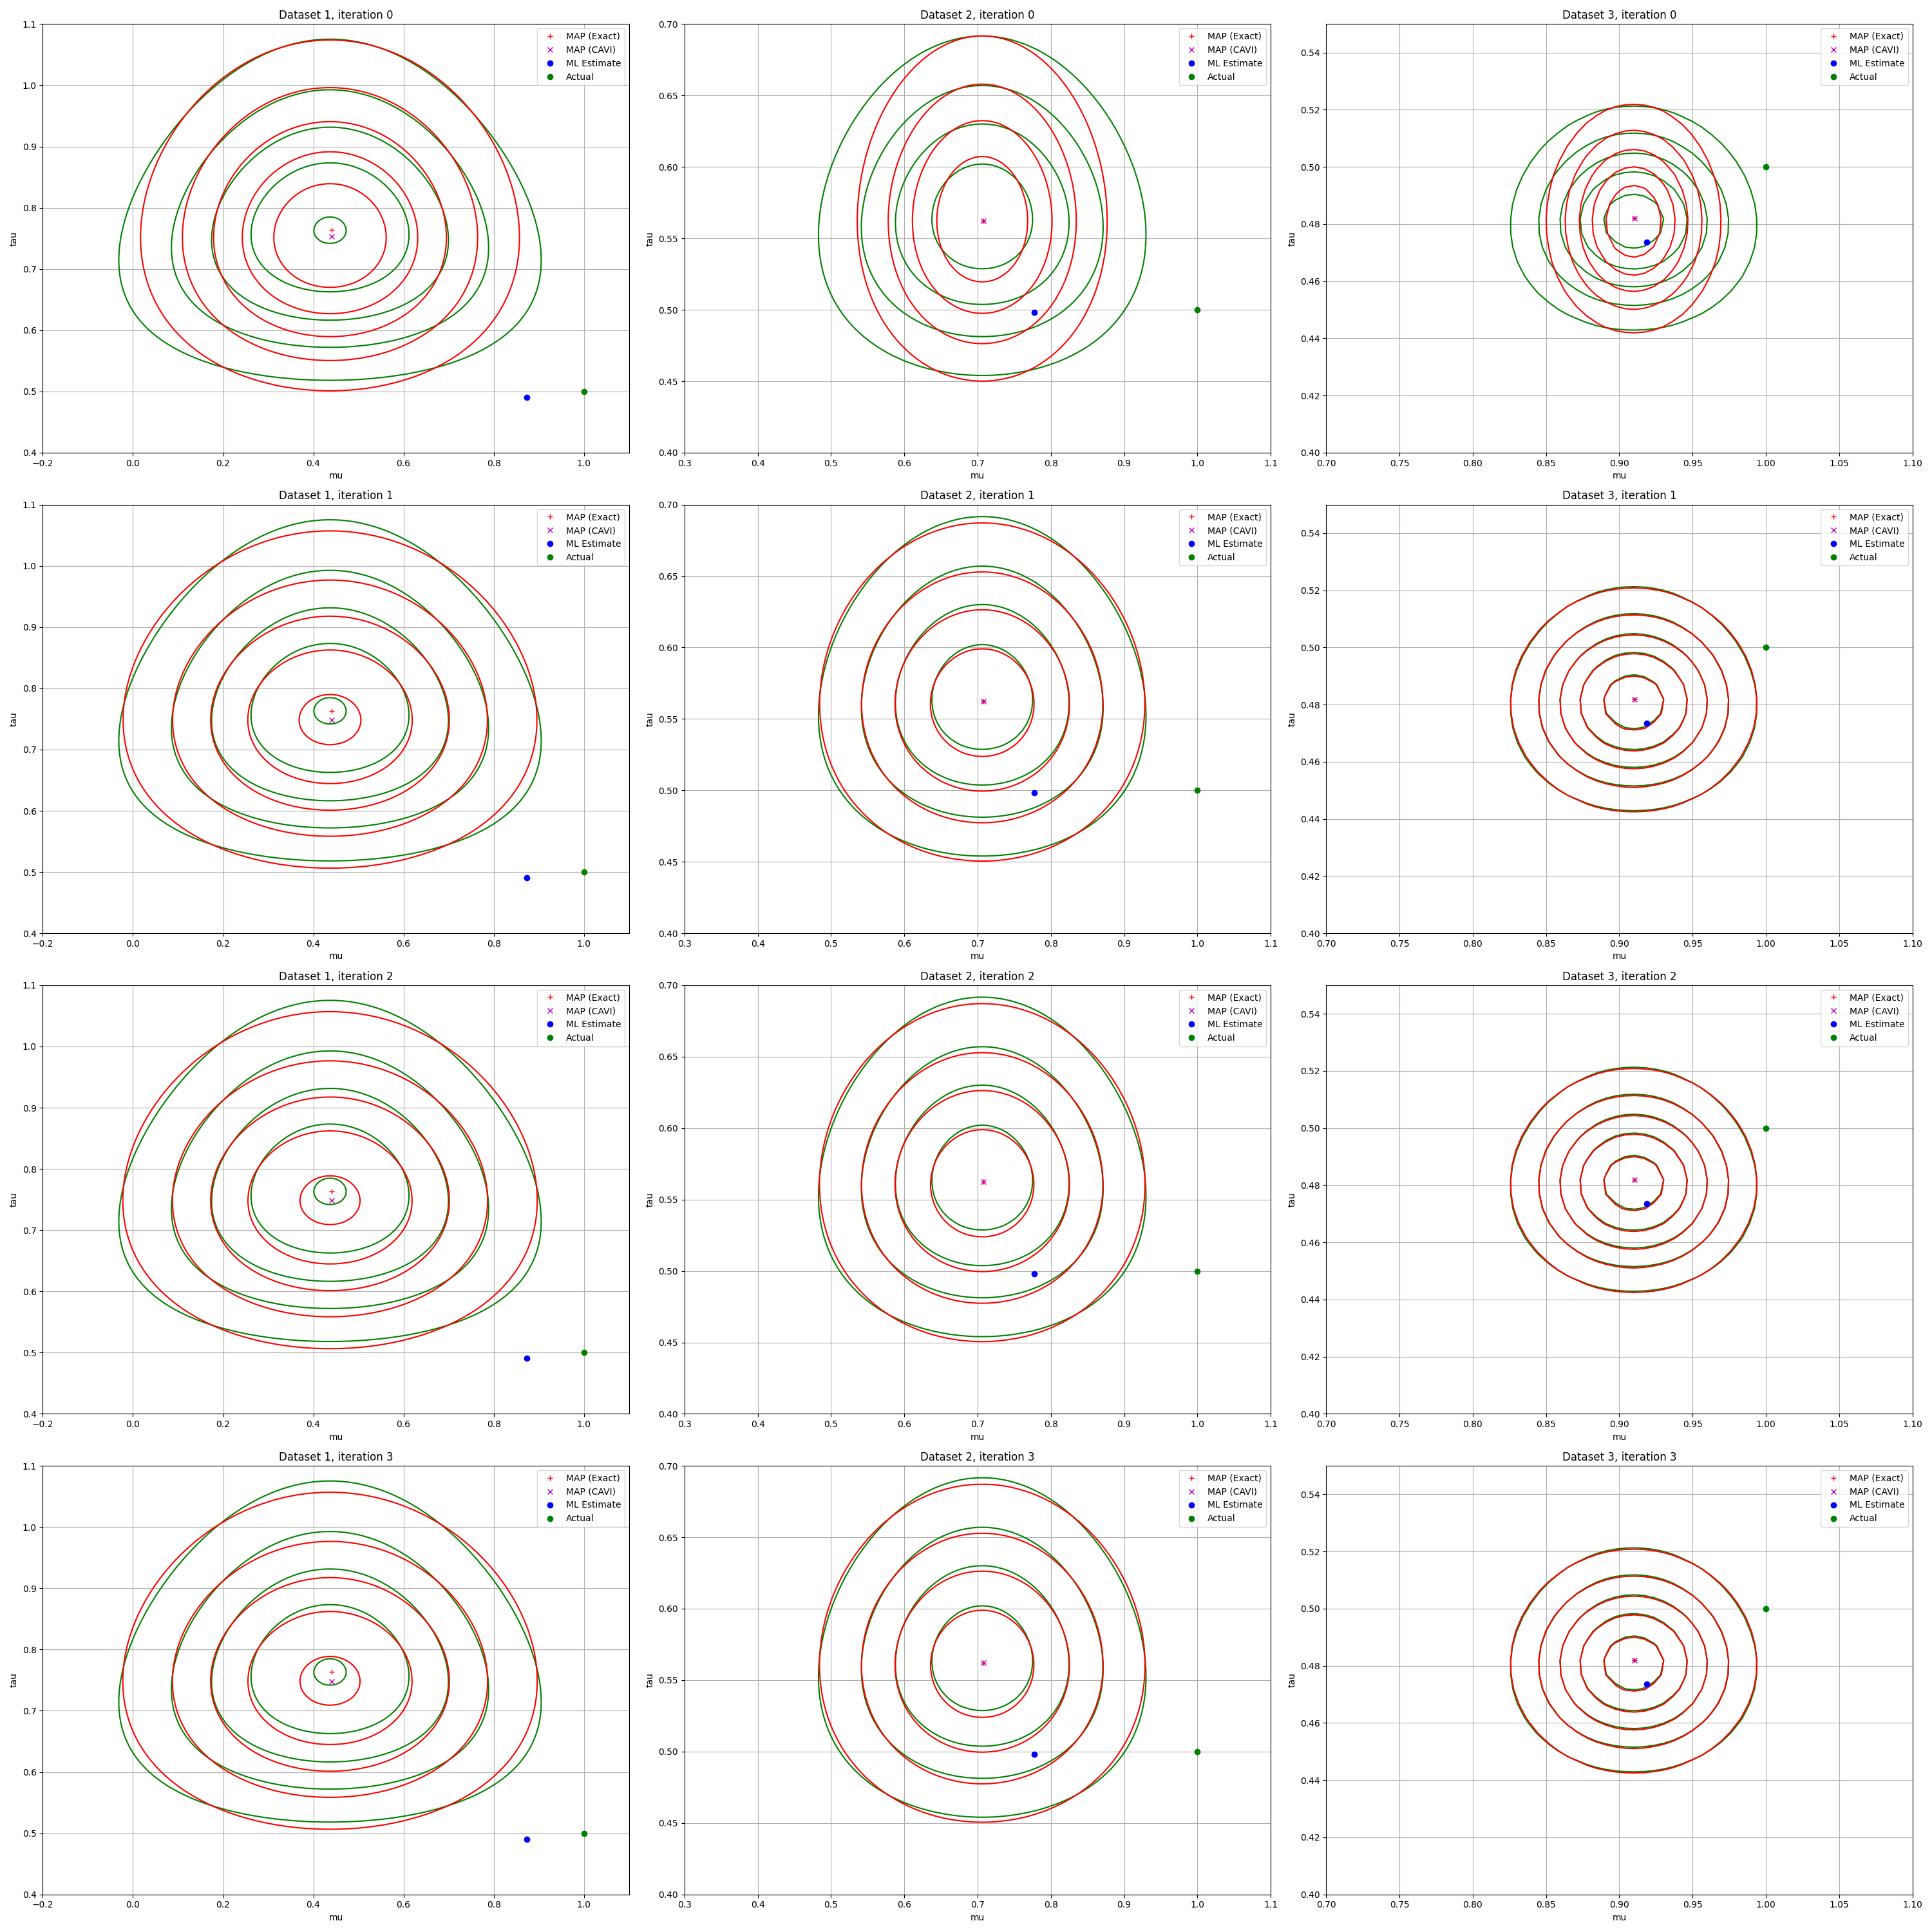
\includegraphics[scale=0.2]{images/15_contours.png}
    \caption{Contours of the approximations by VI and the exact posterior by datasets, by iterations}
    \label{fig:3.15.1}
\end{figure}

And we obtain an elbo plot :
\begin{figure}[H]
    \centering
    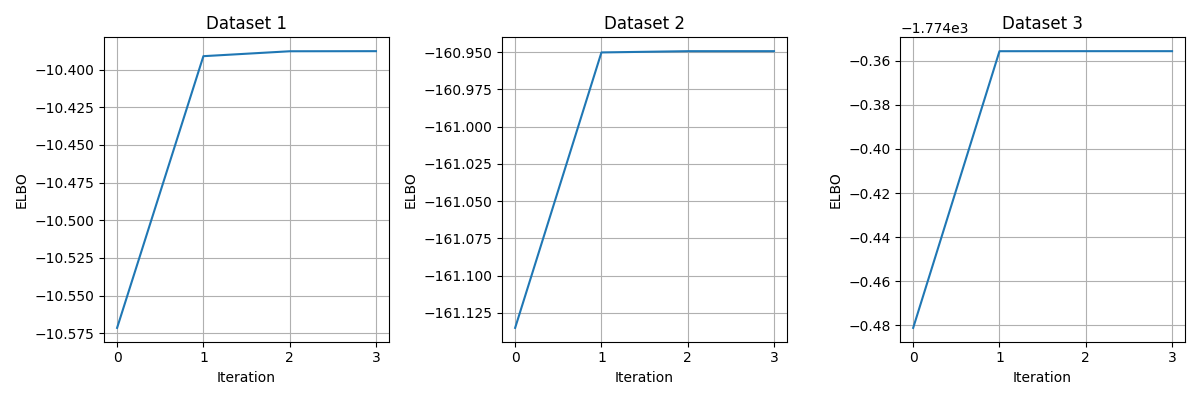
\includegraphics[scale=0.5]{images/15_elbo.png}
    \caption{ELBO plot by datasets}
    \label{fig:3.15.2}
\end{figure}

The code is in appendix \ref{appendix:code.3.15}.

\section{SVI - LDA}

\subsection*{Question 4.16}

According to the Hoffman paper, the local hidden variables are ...

\subsection*{Question 4.17}

In this figure the global variables are ... and the local hidden variables are ...

\subsection*{Question 4.18}

The ELBO formula is:
\begin{equation}
    \mathcal{L}(q) = \mathbb{E}_{q(\theta, z, \beta)}[\log p(w, \theta, z, \beta)] - \mathbb{E}_{q(\theta, z, \beta)}[\log q(\theta, z, \beta)]
\end{equation}
And here we recall that we have:
\begin{equation}
    p(w,z,\theta,\beta) = \prod_{k=1}^{K}p(\beta_k) \prod_{d=1}^{D}p(\theta_d) \prod_{d=1}^{D}\prod_{n=1}^{N}p(z_{dn}|\theta_d)p(w_{dn}|\beta_{z_{dn}})
\end{equation}
Therefore we have:
\begin{equation}
    \begin{split}
         & \mathbb{E}_{q(\theta, z, \beta)}[\log p(w, \theta, z, \beta)]                                                                                                                                                             \\
         & = \mathbb{E}_{q(\theta, z, \beta)}\left[\sum_{k=1}^{K}\log p(\beta_k) + \sum_{d=1}^{D}\log p(\theta_d) + \sum_{d=1}^{D}\sum_{n=1}^{N}\log p(z_{dn}|\theta_d)p(w_{dn}|\beta_{z_{dn}})\right]                               \\
         & \qquad\qquad - \mathbb{E}_{q(\theta, z, \beta)}\left[\sum_{k=1}^{K}\log q(\beta_k) + \sum_{d=1}^{D}\log q(\theta_d) + \sum_{d=1}^{D}\sum_{n=1}^{N}\log q(z_{dn}|\theta_d) + \log q(w_{dn}|\beta_{z_{dn}})\right]          \\
         & = \sum_{k=1}^{K}\mathbb{E}_{q(\beta_k)}[\log p(\beta_k)] + \sum_{d=1}^{D}\mathbb{E}_{q(\theta_d)}[\log p(\theta_d)] + \sum_{d=1}^{D}\sum_{n=1}^{N}\mathbb{E}_{q(z_{dn})}[\log p(z_{dn}|\theta_d) + \log p(w_{dn}|\beta_{z_{dn}})] \\
         & \qquad\qquad + \sum_{k=1}^{K}\mathbb{H}_q[\beta_k] + \sum_{d=1}^{D}\mathbb{H}_q[\theta_d] + \sum_{d=1}^{D}\sum_{n=1}^{N}\mathbb{H}_q[z_{dn}|\theta_d] + \mathbb{H}_q[w_{dn}|\beta_{z_{dn}}]                               \\
    \end{split}
\end{equation}

\newpage
\appendix

\section{Appendix}
\subsection{Question 3.12}\label{appendix:code.3.12}
\lstinputlisting[label = {alg:3.12}]{py_files/3.12.py}

\subsection{Question 3.13}\label{appendix:code.3.13}
\lstinputlisting[label = {alg:3.13}]{py_files/3.13.py}

\subsection{Question 3.14}\label{appendix:code.3.14}
\lstinputlisting[label = {alg:3.14}]{py_files/3.14.py}

\subsection{Question 3.15}\label{appendix:code.3.15}
\lstinputlisting[label = {alg:3.15}]{py_files/3.15.py}

\end{document}